%
%
%
%
%

\begin{figure}
\centering
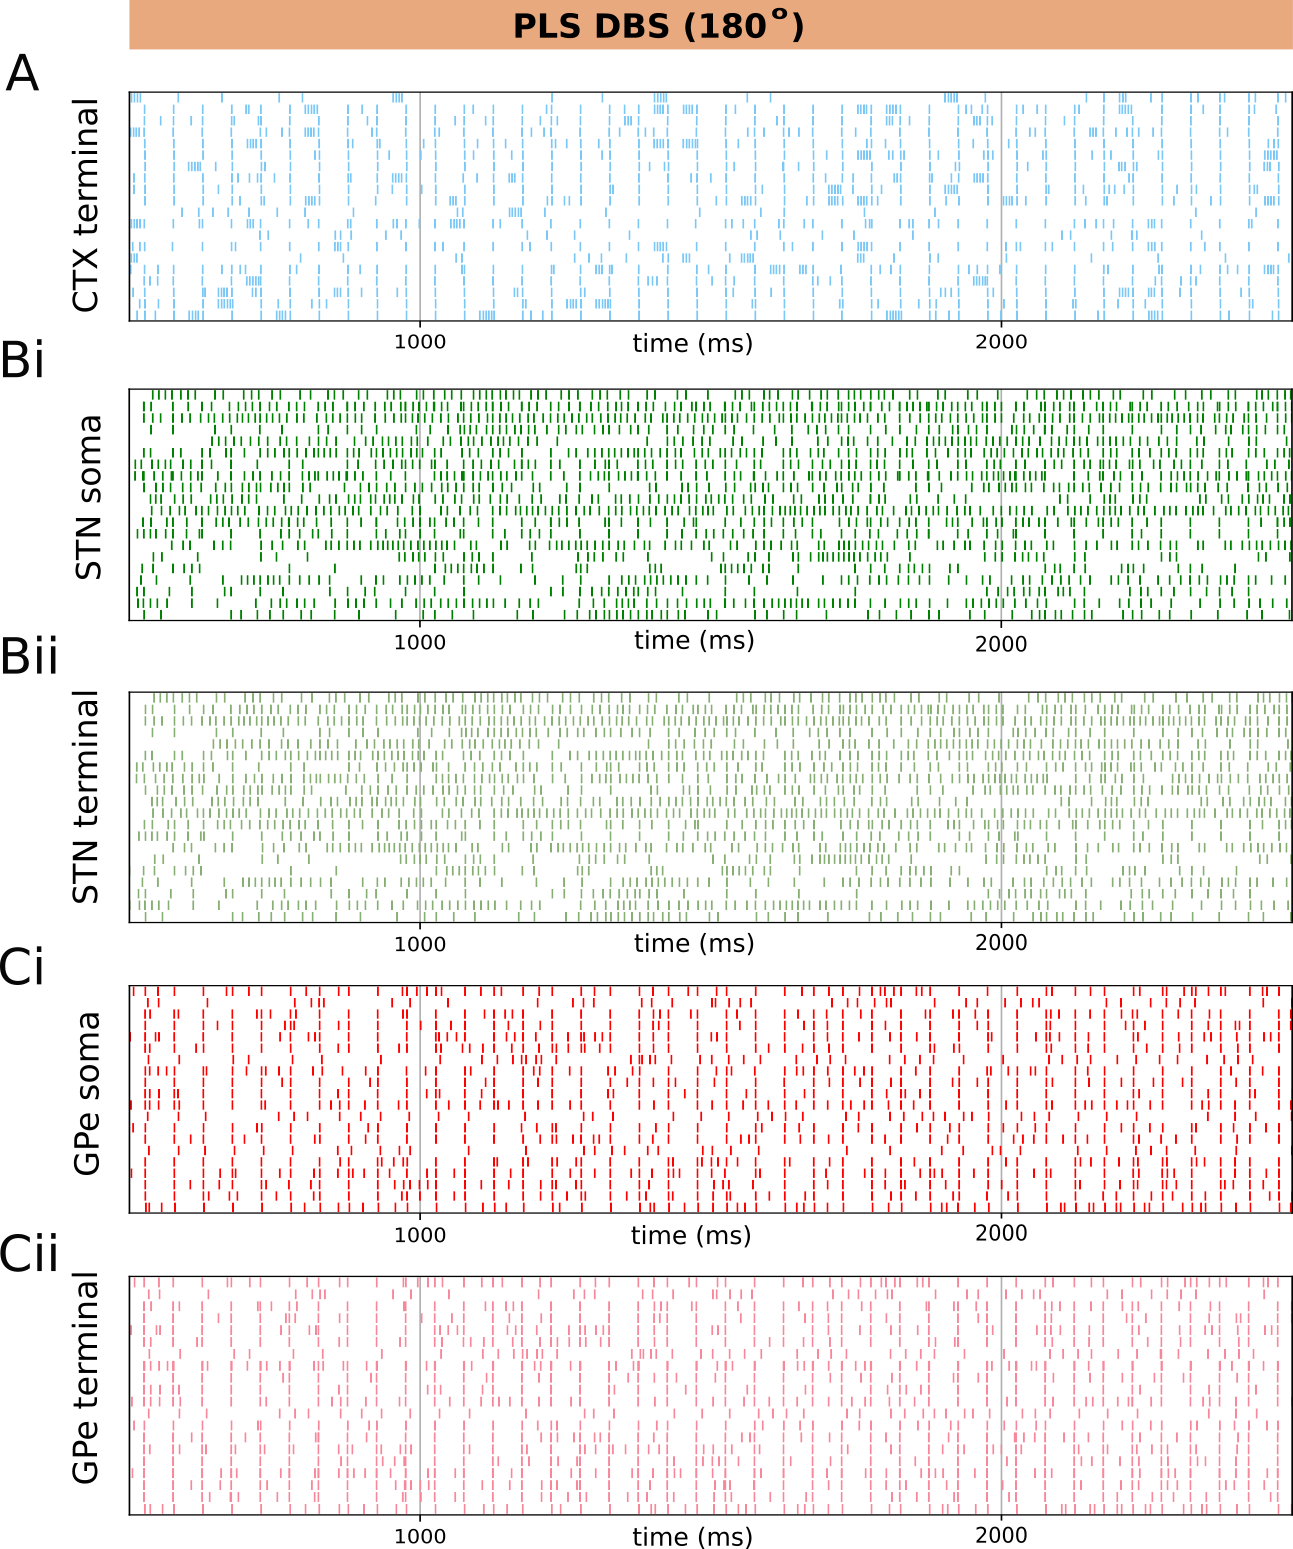
\includegraphics[width=\textwidth]{ch_appendix/figs/fig_pls_ang-180_rastergrams.png}
\caption{
\textbf{Somatic and axonal activation by PLS DBS with \ang{180} phase shift}
DBS pulses were administered with a \ang{180} phase shift with respect to the onset of periodic cortical bursts (20 Hz).
\textbf{A-C}: Representative spike trains recorded at somatic and axon terminal compartments the CTX (A, blue), STN (B, green) and GPe (C, red) populations. PLS DBS was applied during the entire period shown.
}
\label{fig:pls_ang-180_rastergrams}
\end{figure}

\begin{figure}
\centering
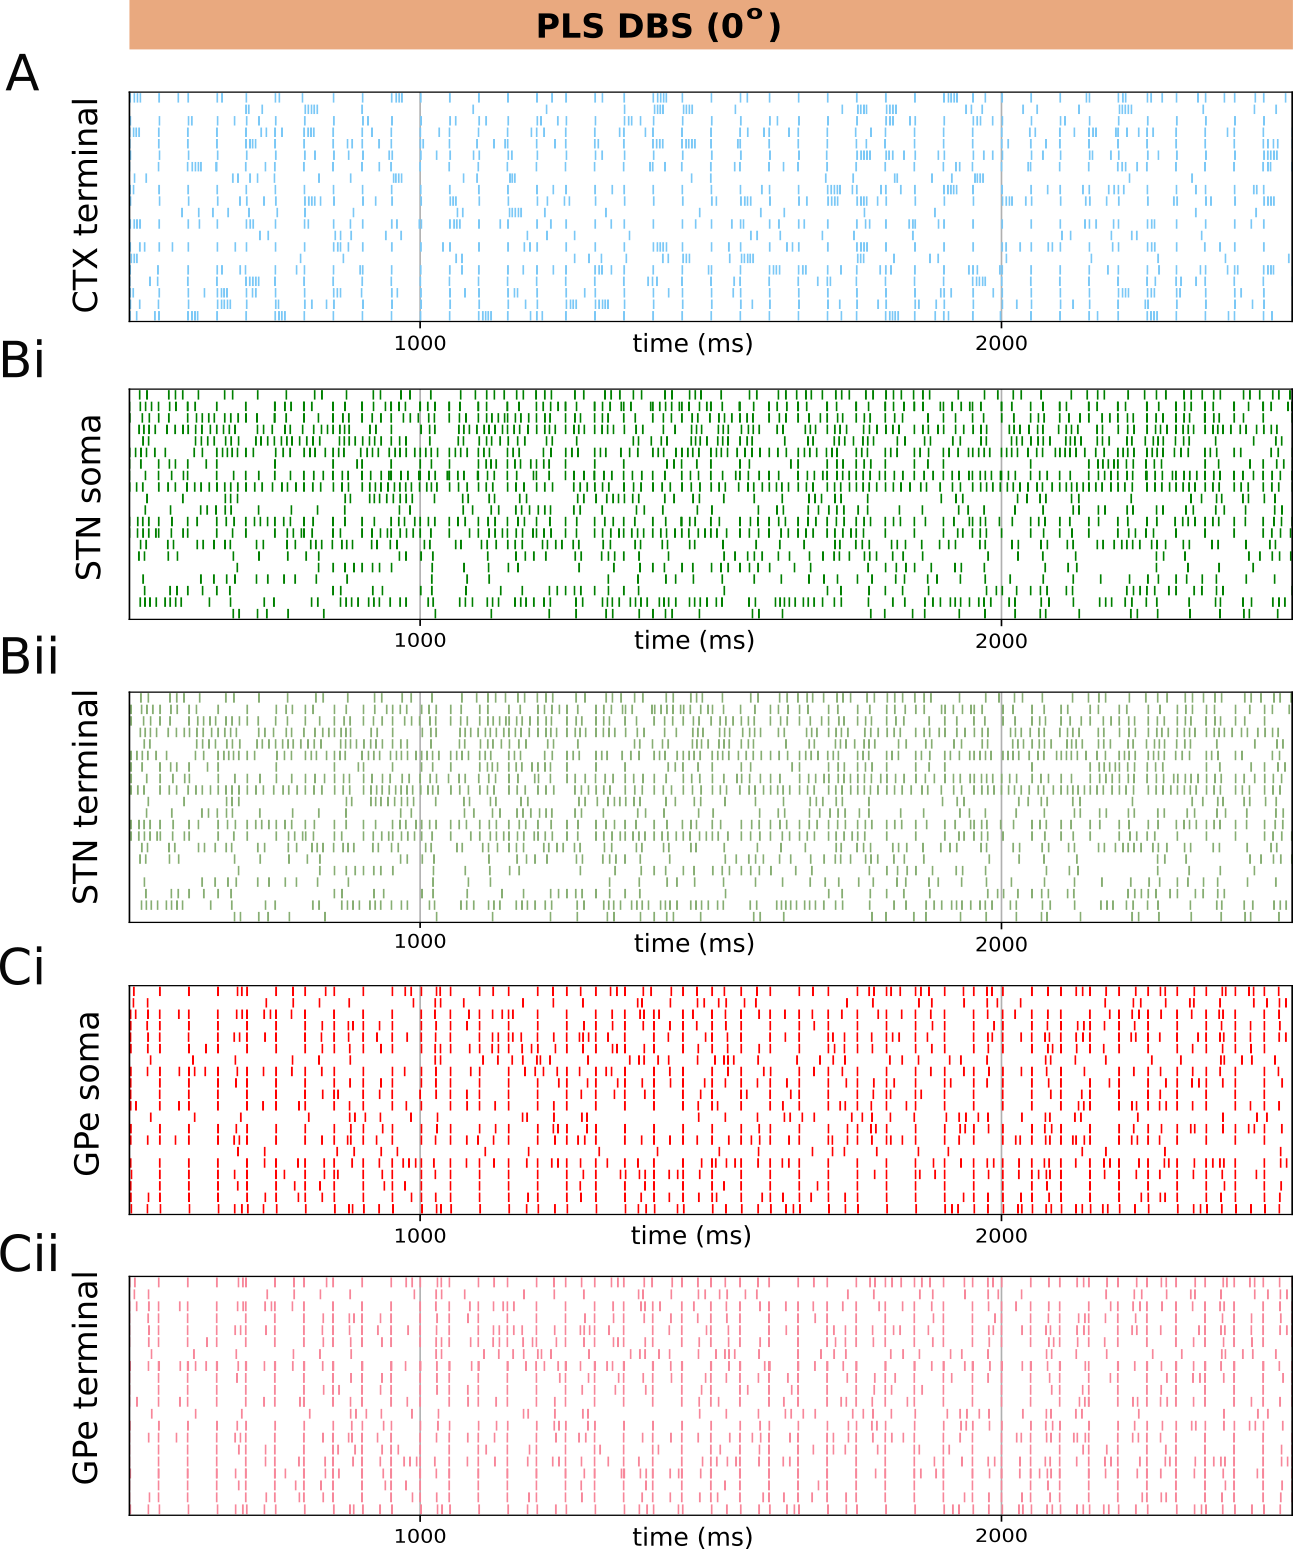
\includegraphics[width=\textwidth]{ch_appendix/figs/fig_pls_ang-0_rastergrams.png}
\caption{
\textbf{Somatic and axonal activation by PLS DBS with \ang{180} phase shift}
DBS pulses were aligned (\ang{0} phase shift) with the onset of periodic cortical bursts (20 Hz).
\textbf{A-C}: Representative spike trains recorded at somatic and axon terminal compartments the CTX (A, blue), STN (B, green) and GPe (C, red) populations. PLS DBS was applied during the entire period shown.
}
\label{fig:pls_ang-0_rastergrams}
\end{figure}